\documentclass[10pt,a4paper]{article}
\usepackage[margin=18mm]{geometry}
\usepackage{amsmath,booktabs,graphicx,tabularx}
\usepackage[hidelinks]{hyperref}
\setlength{\parindent}{0pt}
\setlength{\parskip}{5pt}
\begin{document}
\begin{center}
{\Large Incidence operators and codes: manuscript lengths}\\[4pt]
Whole common theory, two complete applications, and declared proof inputs
\end{center}

The two complete sources contain $@TOTAL_SOURCE@$ nonspace characters in the fixed
primary coordinate. The entire common paper and both complete applications contain
$@TOTAL_WRITTEN@$. Thus the whole manuscript factor is
\[
 \frac{c(L050)+c(F017)}{c(U)+c(A_{L050})+c(A_{F017})}
 =\frac{@C_L050@+@C_F017@}{@C_U_LCD@+@C_A_L050@+@C_A_F017@}
 =\boxed{@WRITTEN@}.
\]
\textbf{This is expansion: the complete replacement is longer.}
There is no achieved whole-topic compression in this coordinate. The factor is
source length divided by replacement length; a factor below one means expansion.

The primary coordinate is NFC nonspace characters in the accepted calibrated
selected extraction. Whole manuscripts include titles, abstracts, tables, proof
and algorithm prose, footnotes and references. Only precisely identified running
furniture is removed. There are no executable listings in these five PDFs, so
symmetric listing exclusion removes no passages here.

\begin{center}
\begin{tabular}{lrr}\toprule
Complete document & Physical pages & Primary length\\\midrule
@DOCROWS@
\bottomrule\end{tabular}
\end{center}

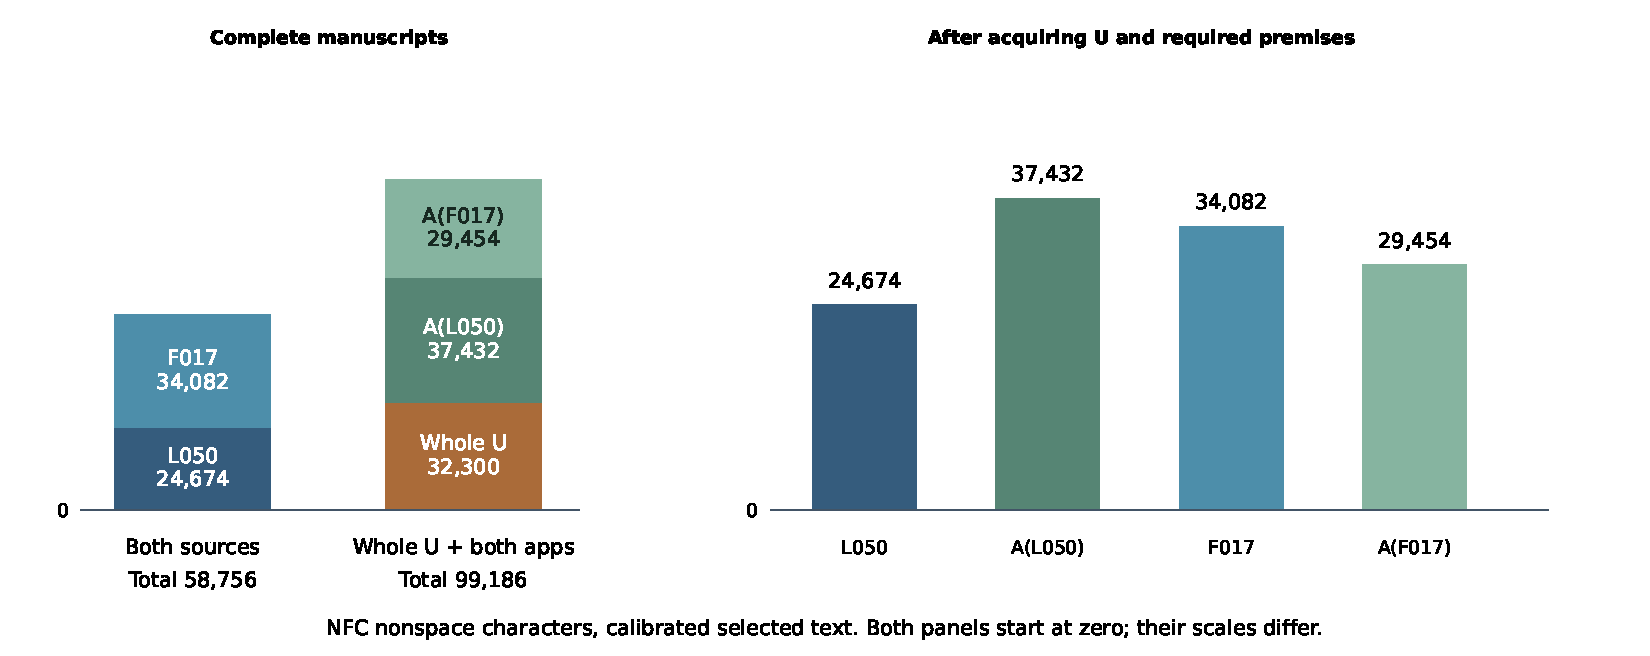
\includegraphics[width=\linewidth]{costs.pdf}

After acquiring the \emph{whole} common paper, the complete declared required
program/data/record collection, and the actual retained mathematical premises,
the conditional comparisons are
\[
 \frac{c(L050)}{c(A_{L050})}=\frac{@C_L050@}{@C_A_L050@}=\boxed{@L050@},\qquad
 \frac{c(F017)}{c(A_{F017})}=\frac{@C_F017@}{@C_A_F017@}=\boxed{@F017@}.
\]
The L050 application is longer than its source; the F017 application is shorter
only in this conditional comparison. Neither comparison discards the initial
acquisition or substitutes for the whole-topic result. No sibling application
is a proof premise. Optional validation is not a required premise.

{\small L050: D. Leemans and B. G. Rodrigues, \emph{Linear codes with complementary duals
from some strongly regular subgraphs of the McLaughlin graph}, Mathematical
Communications 21 (2016), 239--249. F017: J. D. Key and B. G. Rodrigues,
\emph{LCD codes from adjacency matrices of graphs}, complete seventeen-page
author manuscript dated 4 August 2017.}

\newpage
\begin{center}{\Large What must be acquired}\end{center}

The entire fourteen-page common paper is paid once, including interfaces unused
by a particular local application. The fifteen-page L050 and twelve-page F017
applications are both paid in the whole comparison. In the displayed order,
cumulative manuscript costs are $@STAGES@$ (whole common; common plus L050;
common plus both applications). This order is a cost accounting convention,
not a claim about chronological discovery or a minimal proof dependency graph.

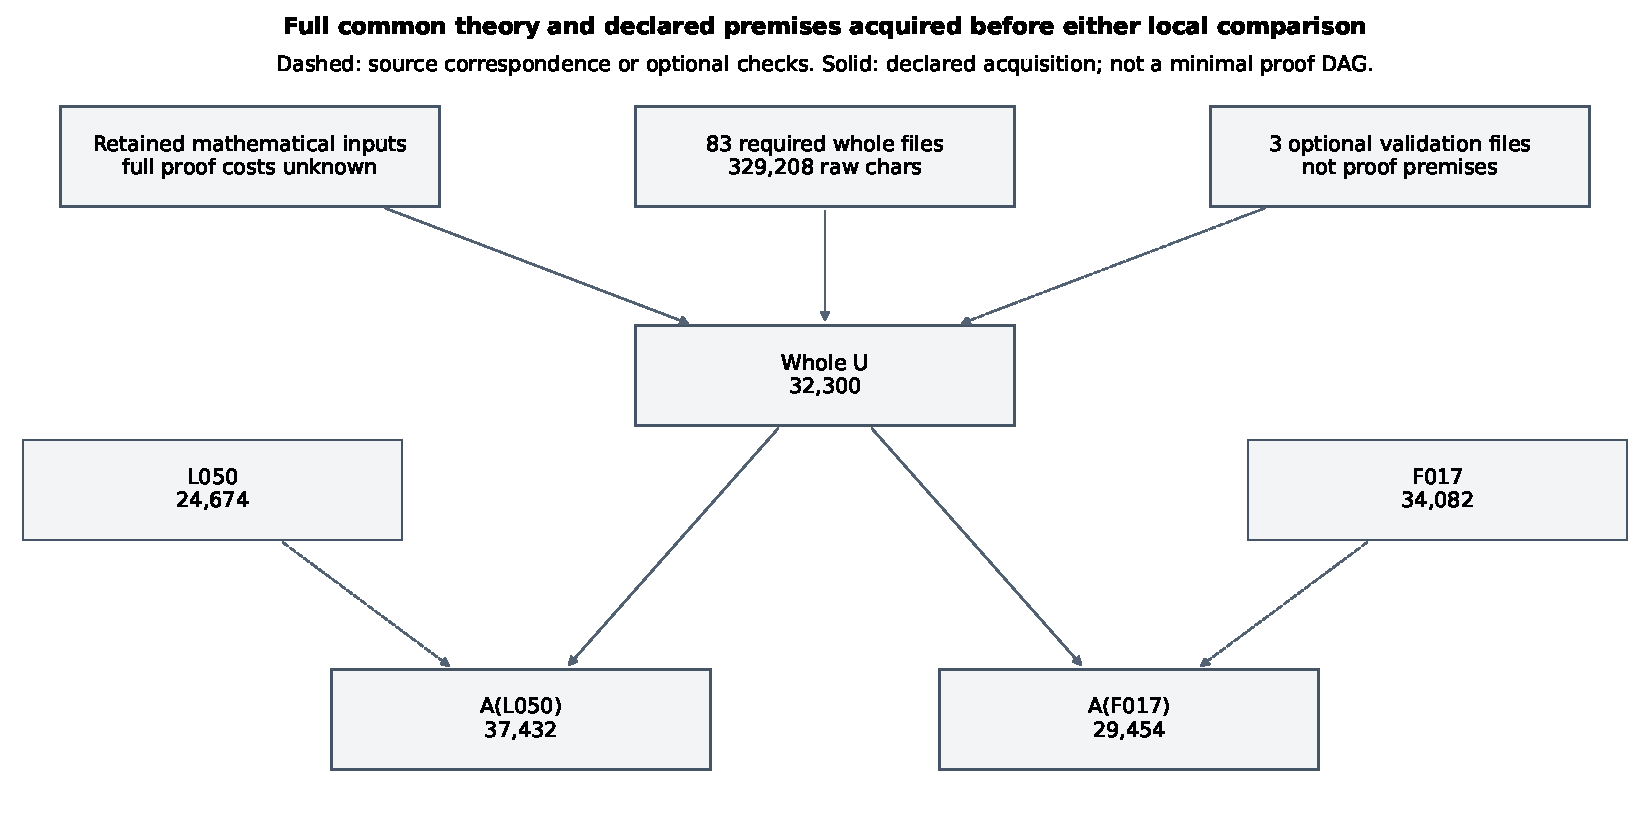
\includegraphics[width=\linewidth]{document_graph.pdf}

The conditional convention conservatively acquires the \emph{complete topic-wide}
required union: 83 unique whole files occupying @REQUIRED_BYTES@ original bytes.
It includes 20 programs, two generated certificates, 19 mandatory data files and
42 retained finite records. No claim is made that every one of these files is
necessary for each individual application. Required computations are not
relabelled as optional, and completed enumeration records remain premises.
The numerical replay does not rerun those enumerations.

\begin{center}\small
\begin{tabular}{lrrr}\toprule
Whole-file role & Files & Original bytes & NFC nonspace chars\\\midrule
@RAWROWS@
\midrule
All unique complete contents & 102 & @RAW_TOTAL@ & @RAW_CHARS@\\
\bottomrule\end{tabular}\end{center}

All 127 occurrences are disclosed; exactly byte-identical complete contents are
counted once within this topic. The three optional validation files are two
programs and an auxiliary JSON file. Eleven operational drivers and five
partial-formal files are separate from mathematical premises. The two Lean
source files and three scope files concern the same nine generic declarations;
they do not formalize both complete sources.

Historical source software, full retained classical proofs, graphics/layout,
external libraries and complete formalization have unknown costs. These are
\emph{unknown, not zero}. The raw inventory is not added to a manuscript
comparison and no software-inclusive factor is reported. Full paths, hashes,
roles, duplicate occurrences and all ten raw-file metric coordinates are
available in the accompanying JSON and CSV files.

\newpage
\begin{center}{\Large Sensitivity and limits}\end{center}

All thirty fixed policy coordinates are retained: three extraction variants,
NFC and NFKC, and five units. Each has one whole manuscript fraction and two
conditional fractions, stored as exact integers and reduced fractions. The
following five-unit table uses calibrated selected NFC text.

\begin{center}\small
\begin{tabular}{lrrr}\toprule
Unit & Whole & L050 conditional & F017 conditional\\\midrule
@SENSITIVITY@
\bottomrule\end{tabular}\end{center}

\begin{center}\small
\begin{tabular}{lrrr}\toprule
Nonspace-character variant & Whole & L050 conditional & F017 conditional\\\midrule
@VARIANTROWS@
\bottomrule\end{tabular}\end{center}

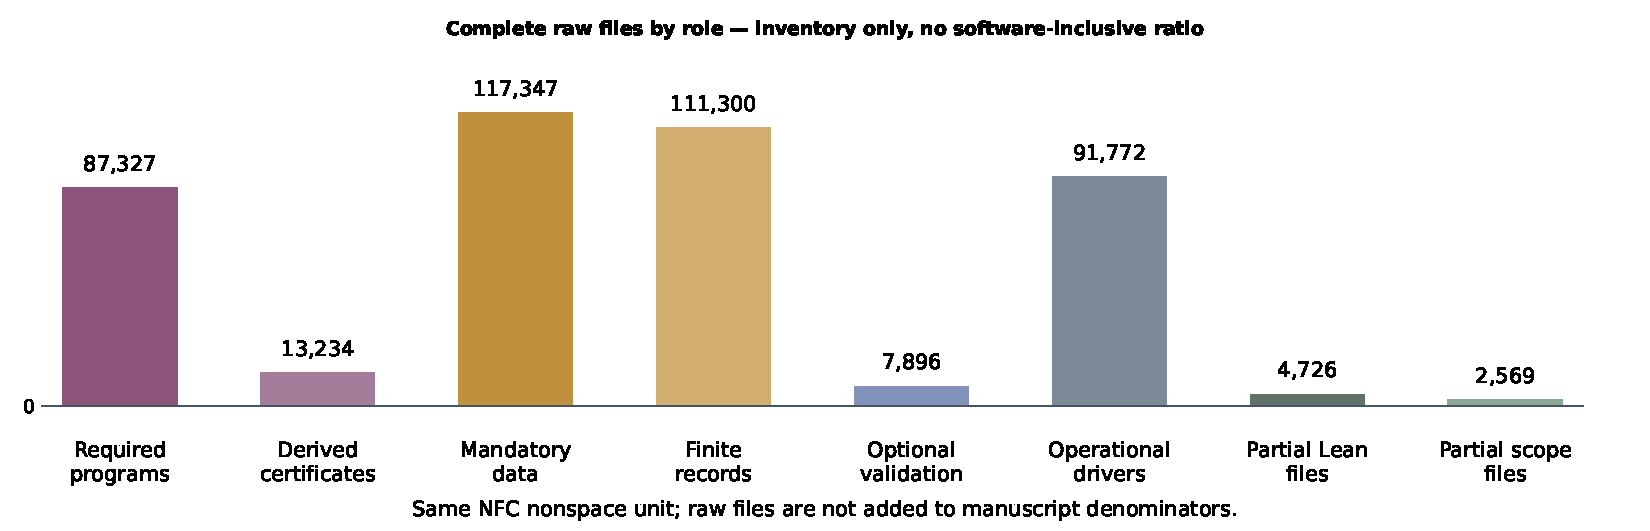
\includegraphics[width=\linewidth]{inventory.pdf}

Raw untrimmed text is the literal PDF extractor output, including furniture;
raw selected text removes only the accepted furniture; calibrated selected text
also makes the accepted occurrence-bound glyph repairs. Printed hyphens remain.
The accepted audit binds actual font dictionaries and events, and preserves the
explicit Type0 extraction qualification. These are extracted-text coordinates,
not full visual or graphic-complexity measurements. Physical extent remains
28 source pages and 41 replacement pages.

The applications recover the \emph{corrected} accepted contracts: 54 L050 and
104 F017 dispositions. Named graph identifications, classification/Brauer inputs,
earlier code results and the seven declared F017 input classes remain attributed
and retained. Four large Paley pairs retain source upper bounds. The source
questions about all SRG$(253,140,87,65)$, the other fifteen-dimensional modules,
general further families and efficient decoding are not newly solved here.
The source maps preserve the exact corrections and qualifications; comparing
lengths does not validate a false literal source statement.

This numerical edition reuses the separately accepted scientific and input
packets. It supplies no new original, question or formalization credit.
Its checks reproduce the integer arithmetic, complete inventory, tables and
actual vector bars; they do not replace the underlying mathematical reviews.
\end{document}
